\section{Результаты}
\label{sec:results}

Все числа раздела получены в полном прогоне \code{scripts/kaggle\_run.sh all}
на GPU T4 (seed 42) на 29.1 млн событий Listen+ и словаре 630\,974 айтема.
Обучение базовой модели сопровождается редкими шагами с нефинитной нормой
градиента: такие шаги пропускаются без обновления весов, обучение
продолжается, а число пропущенных шагов фиксируется в логе. На итоговые
метрики это влияет не более чем на длину обучения.

\subsection{Базовая модель}

Обучение устойчиво: лосс sampled softmax падает с 9.40 (что близко к
$\log 8193 \approx 9.01$ --- уровню инициализации при 8192 негативах) до
6.9--7.1 к 3000-му шагу, а NDCG@10 на валидационном дне растёт монотонно
(рис.~\ref{fig:training}). К концу обучения скорость роста замедляется,
поэтому чекпоинт выбирается по валидации (шаг 2500, NDCG@10 0.0640), а не
по последнему шагу: на нём лосс ниже, но метрика не лучше.

\begin{figure}[t]
\centering
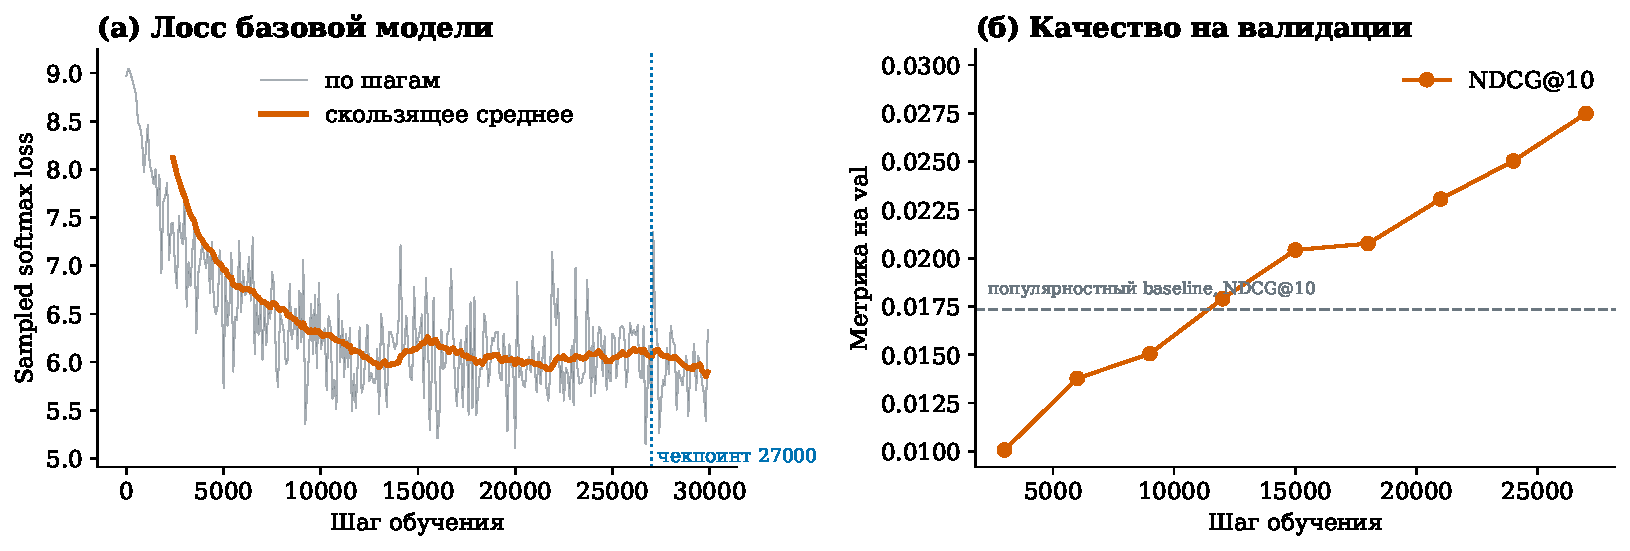
\includegraphics[width=\textwidth]{figures/fig_training.pdf}
\caption{Обучение базовой модели. (а) Лосс sampled softmax: сырые значения и
скользящее среднее по 25 шагам. (б) Метрики на валидационном дне; пунктир ---
NDCG@10 популярностного baseline.}
\label{fig:training}
\end{figure}

\begin{table}[t]
\centering
\caption{Тестовый день, полный каталог (630\,974 айтема), 4\,600
пользователей. SASRec --- опубликованное значение официального бенчмарка
Yambda-50M~\cite{sasrec}, мы его не переобучали.}
\label{tab:test}
\small
\begin{tabular}{@{}lrrrrrr@{}}
\toprule
Модель & NDCG@10 & NDCG@100 & Recall@10 & Recall@100 & MAP@10 & Cov.@100 \\
\midrule
Популярность      & 0.0173 & 0.0227 & 0.0070 & 0.0346 & 0.0078 & 0.011\% \\
Базовая GPT-2     & \textbf{0.0623} & \textbf{0.0802} & \textbf{0.0333} & \textbf{0.1157} & \textbf{0.0328} & 3.4\% \\
GRPO (наш)        & 0.0052 & 0.0099 & 0.0018 & 0.0188 & 0.0023 & 0.28\% \\
\midrule
SASRec (офиц.)    & 0.0748 & 0.0764 & 0.0325 & 0.1026 & --- & 1.3\% \\
\bottomrule
\end{tabular}
\end{table}

Базовая модель даёт NDCG@10 0.0623 против 0.0173 у популярностного baseline
(таблица~\ref{tab:test}), то есть в 3.59 раза лучше; по Recall@100 разрыв
составляет 0.1157 против 0.0346. От опубликованного SASRec базовая модель
отстаёт по NDCG@10 в 1.20 раза и превосходит его по Recall@100 (0.1157
против 0.1026) при заметно меньшем бюджете обучения: 81.6 млн параметров,
4 слоя и около четырёх минут на T4 против публичной конфигурации SASRec.
Сравнение с SASRec мы приводим как внешнюю точку отсчёта, а не как
утверждение о превосходстве: последовательность обучения, инициализация и
аппаратные условия у двух моделей различаются.

Популярностный baseline занимает Coverage@100 около 0.011\%, потому что
отдаёт один и тот же список всем пользователям. Базовая модель покрывает
3.4\% каталога в топ-100, но рекомендует популярные айтемы: средний
перцентиль популярности выдачи равен 0.999, то есть длинный хвост модель не
исследует. Персонализация при этом присутствует: Jaccard между топ-10 разных
пользователей равен 0.030, NDCG выше популярностного baseline.

\subsection{Reward model}

\begin{table}[t]
\centering
\caption{Reward model на отложенном дне (ансамбль из трёх моделей, 198\,325
пар: 25\% реальные, 25\% hard negatives, 25\% скипы, 25\% случайный
каталог).}
\label{tab:rm}
\small
\begin{tabular}{@{}llrr@{}}
\toprule
Голова & Метрика & Модели (диапазон) & Ансамбль \\
\midrule
$r_{\text{listen}}$ & ROC-AUC, случайный каталог & 0.734--0.749 & 0.751 \\
$r_{\text{like}}$   & ROC-AUC, случайный каталог & 0.734--0.749 & \textbf{0.750} \\
                    & ROC-AUC, hard negatives     & 0.544--0.608 & 0.564 \\
                    & AP, hard negatives          & 0.0045--0.0076 & 0.0047 \\
                    & AP, случайный baseline      & 0.0033--0.0039 & 0.0036 \\
                    & ECE, hard negatives         & 0.011--0.012 & 0.009 \\
$r_{\text{sess}}$   & ROC-AUC & 0.556--0.559 & 0.564 \\
$r_{\text{ret}}$    & ROC-AUC & 0.582--0.586 & \textbf{0.596} \\
$r_{\text{ratio}}$  & Spearman, Listen+ & 0.032--0.077 & 0.073 \\
                    & MAE, Listen+ & 0.180--0.278 & 0.214 \\
                    & MAE, вся выборка & 0.426--0.444 & 0.431 \\
\bottomrule
\end{tabular}
\end{table}

Метрики ансамбля сведены в таблице~\ref{tab:rm}. Голова «лайк»
ранжирует случайный каталог с AUC 0.750, а голова «прослушает не меньше
половины» --- с AUC 0.751: обе отделяют реальный исход пользователя от
произвольного трека. Сигнал исчезает, как только кандидаты становятся
правдоподобными: на hard negatives (айтемах из собственной истории
пользователя, которые он не дослушал) AUC головы «лайк» падает до 0.564,
а AP --- 0.0047 против случайного baseline 0.0036. Иными словами, модель
уверенно отличает «хороший трек» от «случайного трека» и почти не отличает
«этот трек пользователь дослушал» от «этот трек он отклонил».

Голова «досмотр» ранжирует долю прослушивания с Spearman 0.073: она
предсказывает средний уровень вовлечённости, но не порядок внутри истории
пользователя. Вспомогательные головы сессии и возврата близки к монетке
(AUC 0.564 и 0.596), что ожидаемо: обе зависят от пользователя и момента,
а не от кандидата; в награде RL они не участвуют.

\begin{figure}[t]
\centering
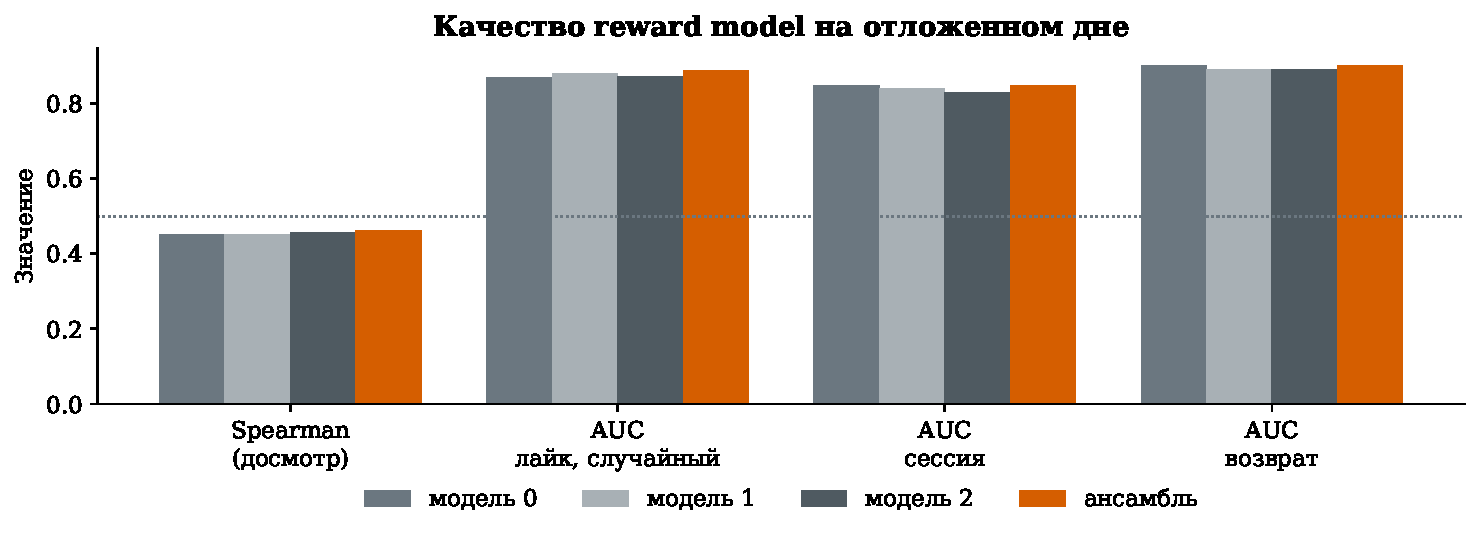
\includegraphics[width=\textwidth]{figures/fig_rm.pdf}
\caption{Качество reward model на отложенном дне. Высота столбцов ---
метрика на отложенном дне; оранжевый --- ансамбль.}
\label{fig:rm}
\end{figure}

Три модели ансамбля согласованы по качеству (разброс AUC меньше 0.02,
рис.~\ref{fig:rm}), но обучены на перекрывающихся подвыборках пользователей
(80\%), поэтому их расхождение отражает различия подвыборок, а не
независимость моделей. Пессимистичный штраф $-\lambda\sigma_r$ смещает
награду на величину порядка одного процента и не ограничивает область, в
которую политика смещается (раздел~\ref{sec:results-rl}).

\subsection{Обучение с подкреплением}
\label{sec:results-rl}

GRPO выполнил 64 шага оптимизатора (1024 промпта, батч 16, группа 8,
горизонт 5). Награда за роллаут выросла с 3.474 на первом шаге до в среднем
3.626 по последним пяти шагам ($+4.4\%$, пик 3.804), KL к опорной политике
прошёл через максимум 0.573 и стабилизировался на 0.10, а число уникальных
айтемов в выдаче упало с 383 до 140 (рис.~\ref{fig:rldyn}). Политика
увеличила оптимизируемую голову и одновременно потеряла разнообразие.

\begin{figure}[t]
\centering
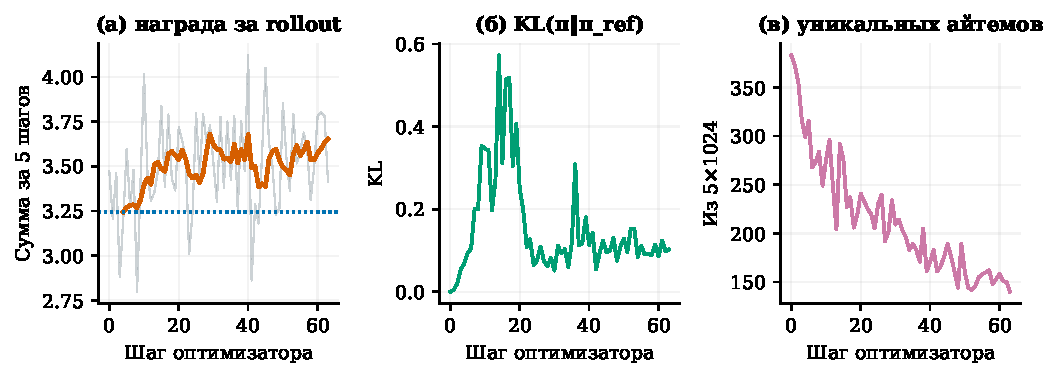
\includegraphics[width=\textwidth]{figures/fig_rl_dynamics.pdf}
\caption{Динамика GRPO. (а) Средняя награда роллаута за шаг: сырые значения
и скользящее среднее; пунктир --- стартовый уровень. (б) KL к опорной
политике. (в) Число уникальных айтемов, выданных на 1024 промпта по
5 шагов: разнообразие падает монотонно.}
\label{fig:rldyn}
\end{figure}

\paragraph{Цена.} На тестовом дне RL-политика даёт NDCG@10 $=0.0052$ против
$0.0623$ у базовой модели, то есть падение на 92\%; Recall@100 падает с
0.1157 до 0.0188 ($-84\%$), MAP@10 --- с 0.0328 до 0.0023.
Парный бутстрэп по 4\,600 пользователям: $\Delta = -0.0230$ для NDCG@10,
95\% CI $[-0.0254,\,-0.0206]$; $\Delta = -0.0471$ для Recall@100,
CI $[-0.0505,\,-0.0438]$; $\Delta = -0.0097$ для MAP@10,
CI $[-0.0111,\,-0.0083]$. Все три интервала лежат ниже нуля с запасом,
эффект не объясняется шумом.

Поведение выдачи меняется согласованно и в одну сторону
(рис.~\ref{fig:behaviour}):
\begin{itemize}[leftmargin=1.2em,itemsep=1pt,topsep=2pt]
  \item средняя длина рекомендованного трека падает с 181 до 124 с
        ($-31\%$) --- короткие треки легче «дослушать»;
  \item Jaccard между топ-10 разных пользователей растёт с 0.030 до 0.736
        ($\times 24.6$): у всех почти один и тот же список;
  \item оценка головы «лайк» в выдаче падает с 0.210 до 0.102 ($-51\%$),
        хотя именно эта голова моделирует явное предпочтение;
  \item оценка головы «досмотр» растёт с 0.531 до 0.598 ($+13\%$) ---
        ровно та голова, которую оптимизировала награда;
  \item доля айтемов из истории пользователя в выдаче падает с 13.2\% до
        2.4\%: политика перестаёт повторять прошлое, но не заменяет его
        релевантным.
\end{itemize}

\begin{figure}[t]
\centering
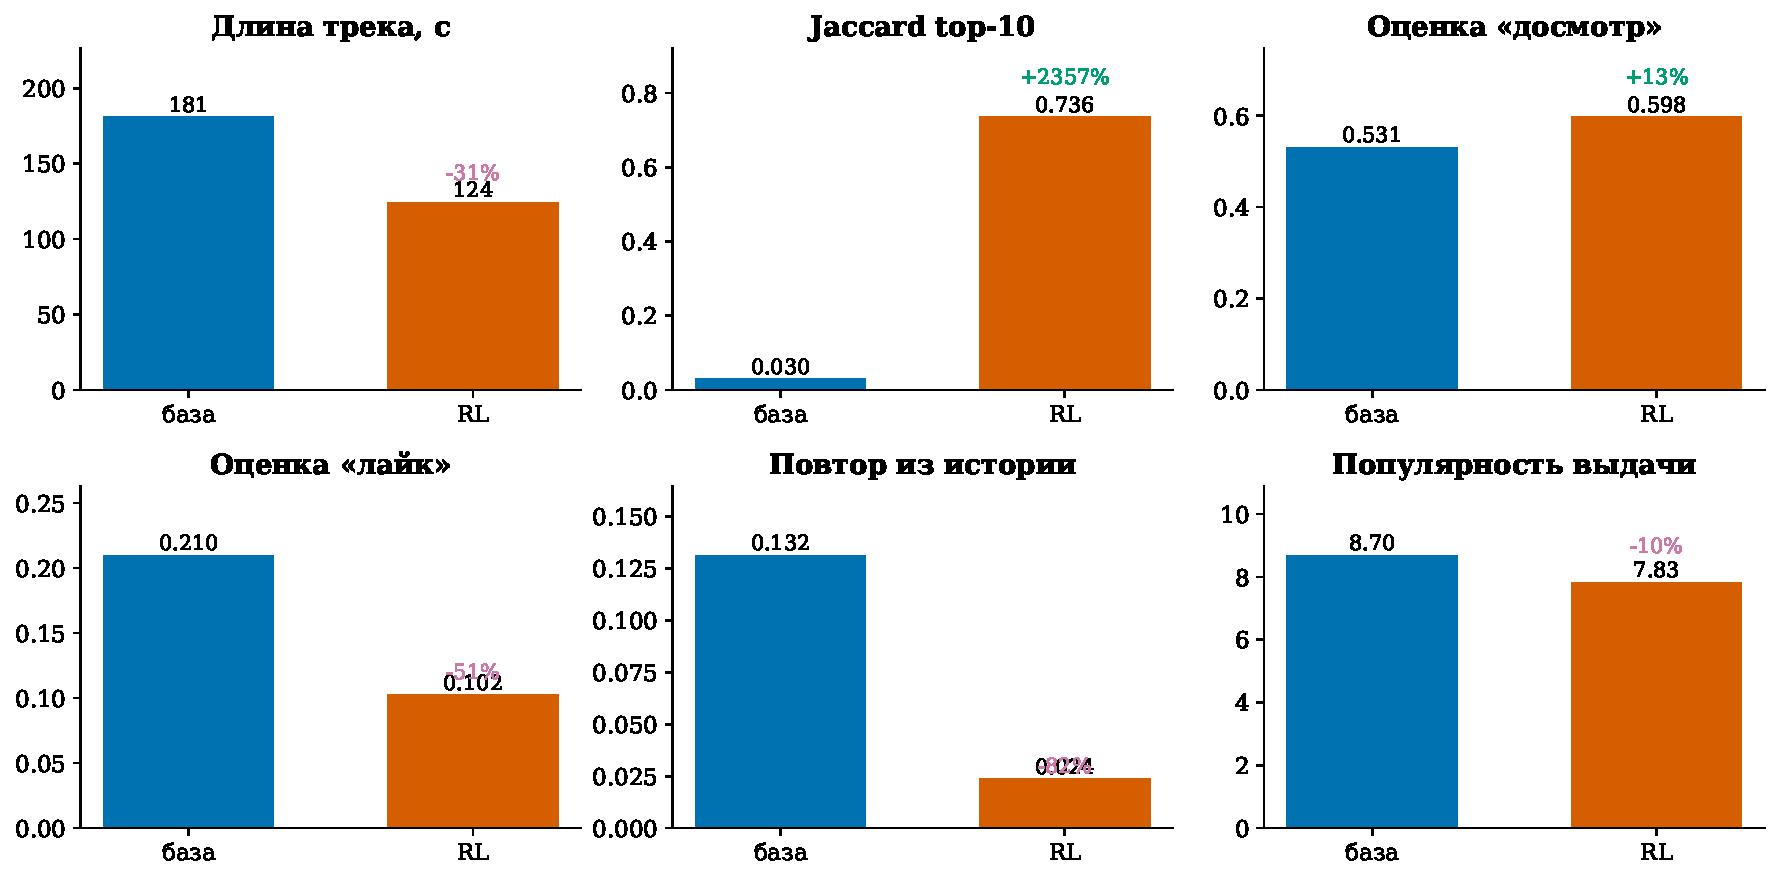
\includegraphics[width=\textwidth]{figures/fig_behavior.pdf}
\caption{Поведение выдачи: базовая модель против RL. Каждая панель ---
отдельная метрика с собственной шкалой; процент над столбцами --- изменение
относительно базы. Расхождение знаков у голов reward model («досмотр»
растёт, «лайк» падает) показывает, что политика оптимизировала одну голову
за счёт другой.}
\label{fig:behaviour}
\end{figure}

По пользователям эффект неоднороден (рис.~\ref{fig:peruser}): NDCG@10
улучшился у 109 человек, не изменился у 3\,765 и ухудшился у 726; по
Recall@100 лучше стало у 231, без изменений у 2\,505, хуже у 1\,864. Провал
в среднем создан пользователями, у которых базовая модель попадала в цели и
RL сломала это попадание; у большинства метрика оставалась нулевой и до RL.

\begin{figure}[t]
\centering
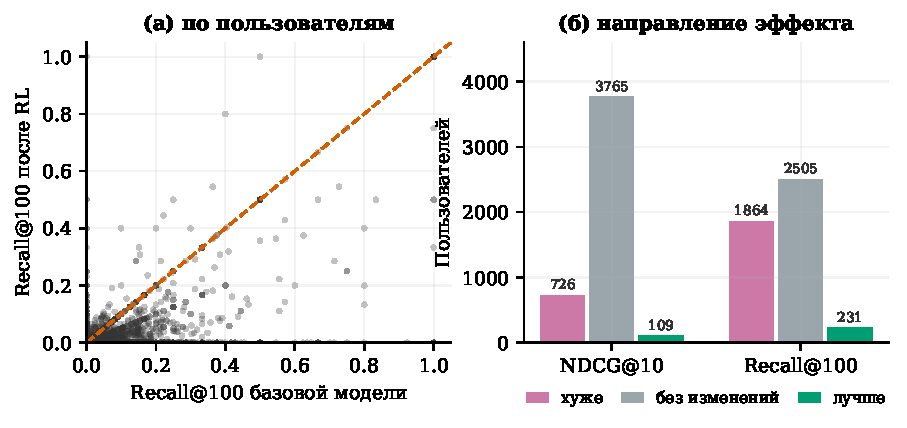
\includegraphics[width=\textwidth]{figures/fig_per_user.pdf}
\caption{Эффект по пользователям. (а) Recall@100 до и после RL; точки ниже
диагонали --- пользователи, которым RL ухудшил выдачу. (б) Направление
эффекта по двум метрикам.}
\label{fig:peruser}
\end{figure}

\subsection{Многошаговая генерация}

При генерации пяти айтемов подряд разнообразие падает у обеих моделей, но
глубоко расходятся они в исходном уровне: у базы уникальных айтемов на
1\,000 роллаутов $172 \to 169$, у RL --- $124 \to 92$. Доля повторов (айтем
уже в истории или уже сгенерирован в этом роллауте) растёт с 7.5\% до 12.0\%
у базы и с 2.0\% до 5.0\% у RL (рис.~\ref{fig:multistep}). RL реже
повторяет историю, но сильнее схлопывается сам с собой --- признак узкого
набора «безопасных» айтемов, который политика присвоила на этапе RL.

\begin{figure}[t]
\centering
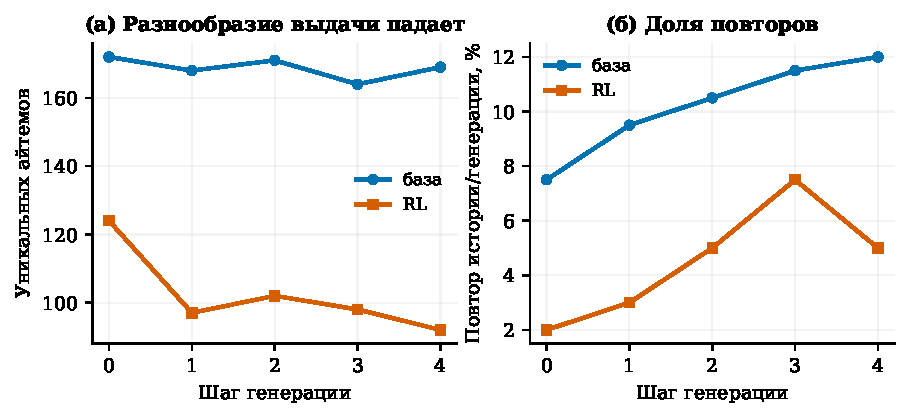
\includegraphics[width=\textwidth]{figures/fig_multistep.pdf}
\caption{Пятишаговая генерация на 1\,000 пользователях. (а) Уникальных
айтемов на шаге. (б) Доля повторов: айтем уже в истории пользователя или
уже сгенерирован в этом роллауте.}
\label{fig:multistep}
\end{figure}

\begin{figure}[t]
\centering
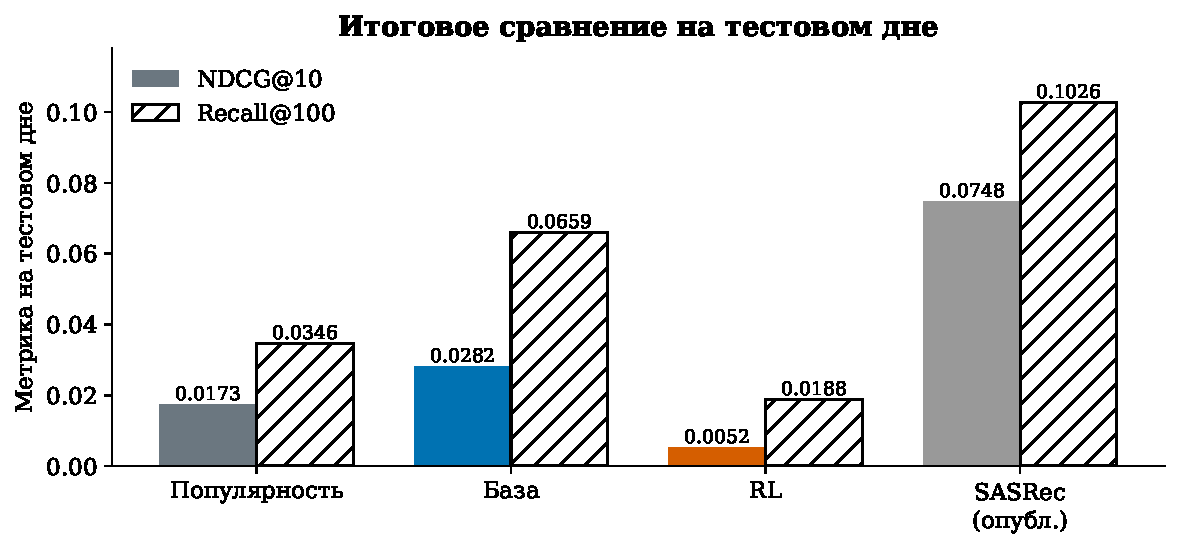
\includegraphics[width=\textwidth]{figures/fig_leaderboard.pdf}
\caption{Итоговое сравнение на тестовом дне. Для каждой модели сверху
сплошной столбец NDCG@10, снизу штрихованный Recall@100. SASRec ---
опубликованное значение, а не наш прогон.}
\label{fig:leaderboard}
\end{figure}

\subsection{Лайки тестового дня}

Like-NDCG@10 у базовой модели равен 0.0055, like-Recall@100 --- 0.0560
на 1\,098 пользователях с лайками и историей Listen+. Эти значения ниже
ранжирования по дослушанным целям (таблица~\ref{tab:test}), что ожидаемо:
лайк --- редкое событие (3.1\% от целей), и модель, обученная на
прослушиваниях, не наводится на него напрямую. Показатель важен тем, что
считается по независимому сигналу, не участвующему в награде RL, и нацелен
на качество списка, поэтому мы используем его как внешний контроль при
обсуждении RL.
